% radiosynth - From MHD to MHz: the story of a thermal free-free radio image
% Copyright (C) 2026 Soumitra Hazra
% Compile with: pdflatex radiosynth_bremsstrahlung_story.tex (twice); needs ff_rays.pdf and ff_profiles.pdf
\documentclass[11pt,a4paper]{article}
\usepackage[T1]{fontenc}
\usepackage{lmodern}
\usepackage[margin=2.6cm]{geometry}
\usepackage{amsmath,amssymb,bm}
\usepackage{booktabs}
\usepackage{graphicx}
\usepackage{xcolor}
\usepackage{enumitem}
\usepackage{needspace}
\usepackage[font=small,labelfont=bf]{caption}
\usepackage[colorlinks=true,linkcolor=blue!50!black,urlcolor=blue!50!black]{hyperref}

\definecolor{accent}{RGB}{31,78,121}
\definecolor{boxbg}{RGB}{236,243,250}
\newcommand{\code}[1]{\texttt{#1}}
\newcommand{\vect}[1]{\bm{#1}}
\newcommand{\dd}{\mathrm{d}}
\newcommand{\kB}{k_\mathrm{B}}
\newcommand{\ncr}{n_\mathrm{cr}}
\newcommand{\rsun}{R_\odot}
\setlength{\parskip}{5pt}
\setlength{\parindent}{0pt}
\setlength{\emergencystretch}{2.5em}
\setlist{itemsep=2pt,topsep=3pt}

\newcommand{\chapterhead}[2]{\needspace{8\baselineskip}\vspace{10pt}{\Large\bfseries\color{accent} #1\par}\vspace{2pt}{\itshape\color{gray} #2\par}\vspace{4pt}}
\newcommand{\keyidea}[1]{\par\smallskip\noindent\colorbox{boxbg}{\parbox{\dimexpr\linewidth-2\fboxsep}{\small\textbf{In one sentence:} #1}}\par\smallskip}

\hypersetup{pdftitle={The story of a radio image},pdfauthor={Soumitra Hazra}}

\begin{document}

\begin{center}
{\LARGE\bfseries\color{accent} The story of a radio image\par}
\vspace{0.25cm}
{\large How \textsf{radiosynth} turns a model of the corona\\ into a picture of the radio Sun (thermal free--free emission)\par}
\vspace{0.4cm}
{\normalsize Soumitra Hazra\par}
{\small \textsf{radiosynth} 2.2.0 --- \emph{From MHD to MHz} --- \url{https://github.com/soumitrahazra/radiosynth}\par}
\end{center}

\vspace{0.3cm}
Imagine you point a radio telescope at the Sun and tune it to 80\,MHz. You see a glowing
disk, a little larger than the Sun you see with your eyes, at a temperature of about a million
degrees. Where does that light come from, and how can a computer predict it from a simulation of
the corona? This short note tells the story, one step at a time, with only the equations that are
really needed.

%----------------------------------------------------------------------
\chapterhead{1.\quad We start at the telescope and walk backwards}{The trick that makes the problem easy}

Light travels from the Sun to the telescope. To make a picture we would have to follow every
bit of light from every point of the corona and see which ones happen to reach us --- hopeless.
So we do the opposite: for every pixel of the image we start a \emph{ray} at the telescope, send
it backwards into the corona, and collect along the way all the light that would travel forward
along the same path into that pixel.

The telescope sits at Earth, 215 solar radii away. Each pixel looks in a slightly different
direction $\vect v$, and its ray starts where it first enters the model. One pixel, one ray, one
number at the end: the brightness of that pixel.

\keyidea{one ray per pixel, traced from the observer into the model.}

%----------------------------------------------------------------------
\chapterhead{2.\quad Where the light is born}{Hot electrons passing by ions}

The corona is a hot, thin gas of electrons and ions, at one to two million kelvin. Every time a
fast electron flies past an ion, it is pulled and deflected, and it radiates a little burst of
radio waves. This is \emph{free--free emission}, or \emph{bremsstrahlung} (``braking
radiation''). Because the electrons move at random, like in any hot gas, the emission is
\emph{thermal}.

A hot gas that emits also absorbs. Two numbers describe it at each point:

\begin{itemize}
\item the \textbf{source function}, the brightness the gas would have if we could see only it, and
      nothing else. For a thermal gas at radio frequencies it is simply proportional to its
      temperature:
      \begin{equation}
        B_\nu=\frac{2\nu^2\kB T_e}{c^2};
      \end{equation}
\item the \textbf{absorption coefficient} $\kappa_\nu$, which says how quickly the gas blocks
      light coming from behind it. Each electron needs an ion nearby, so it grows as the
      \emph{square} of the density; slow electrons interact more, so it falls with temperature;
      and low frequencies are absorbed much more:
      \begin{equation}
        \kappa_\nu\simeq 0.018\,g\,\frac{n_e^2}{\nu^2\,T_e^{3/2}}\ \ \text{cm}^{-1}
        \qquad(n_e\text{ in cm}^{-3},\ \nu\text{ in Hz},\ T_e\text{ in K}),
      \end{equation}
      where $g\approx10$ is the ``Gaunt factor'', a slowly varying number that collects the
      details of the collisions.
\end{itemize}

To get a feeling: in the low corona, $n_e=10^9$\,cm$^{-3}$ and $T_e=1$\,MK, a radio wave of
80\,MHz is weakened by a factor $e$ after only about 360\,km
($\kappa\approx2.8\times10^{-6}$\,m$^{-1}$), while at 1\,GHz it can travel about 56\,000\,km. That is why
the low-frequency Sun is opaque high in the corona, and the high-frequency Sun is transparent.

\keyidea{every point of the corona glows at its own temperature ($B_\nu$) and blocks light
behind it at a rate $\kappa_\nu\propto n_e^2/\nu^2$.}

%----------------------------------------------------------------------
\chapterhead{3.\quad The corona is a lens}{Why the rays do not go straight}

A plasma slows down radio waves of low frequency. Its refractive index is
\begin{equation}
  \mu=\sqrt{1-\frac{n_e}{\ncr}},\qquad
  \ncr\approx1.24\times10^{8}\left(\frac{\nu}{100\,\text{MHz}}\right)^2\ \text{cm}^{-3}.
\end{equation}
$\ncr$ is the \emph{critical density}. Where the density approaches it, $\mu$ drops towards zero;
beyond it ($n_e>\ncr$) the wave cannot exist at all. The corona is densest near the Sun, so
it acts like a lens that pushes the rays \emph{away} from the dense plasma. The direction of the ray
turns according to
\begin{equation}
  \frac{\dd\vect v}{\dd s}=\frac{\nabla\mu}{\mu}-\vect v\left(\vect v\cdot\frac{\nabla\mu}{\mu}\right),
\end{equation}
which simply says: \emph{bend towards where $\mu$ is larger}, i.e.\ towards thinner plasma. A ray
that heads for the Sun slows down, curves, and is reflected before it reaches the critical
surface --- like a ball rolling up a hill and coming back down (Fig.~\ref{fig:rays}). At 80\,MHz
the critical surface of a typical corona lies at about $1.3\,\rsun$, so the rays never get closer
to the Sun than that.

\begin{figure}[ht]
\centering
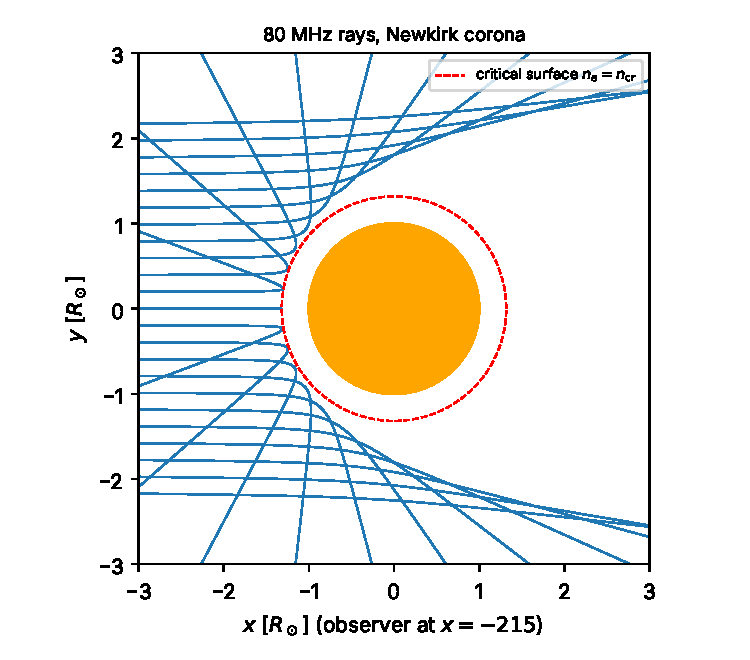
\includegraphics[width=0.5\textwidth]{ff_rays.pdf}
\caption{Rays at 80\,MHz, computed by \textsf{radiosynth}. They come from the telescope on the
left, curve away from the dense plasma and turn around above the critical surface (red dashed).}
\label{fig:rays}
\end{figure}

\keyidea{the denser the plasma, the more the rays bend; they turn back before the critical
density $\ncr\propto\nu^2$.}

%----------------------------------------------------------------------
\chapterhead{4.\quad Walking the ray, one step at a time}{What the computer actually does}

The computer cannot follow a smooth curve; it takes small steps of length $\Delta s$. At each
step, for every ray at once, it does the same few things:

\begin{enumerate}[label=\textbf{\arabic*.}]
\item \textbf{Look half a step ahead.} Go to the middle of the next step,
      $\vect r_{1/2}=\vect r+\vect v\,\Delta s/2$, and read the density, its gradient and the
      temperature of the model there.
\item \textbf{Check that the ray can continue.} Stop if it has left the model, hit the
      photosphere, or run into plasma denser than $\ncr$.
\item \textbf{Make sure the step is small enough.} If the ray would bend too much in one step
      (more than about $1/50$ of a radian), or if it is about to reach the critical surface, shrink
      the step and try again.
\item \textbf{Turn and move.} Rotate the direction by the amount the lens of
      Chapter~3 asks for, and move to the end of the step. Right at the turning point, where the
      path is a small parabola, jump directly to the other side of the parabola. If a ray
      overshoots anyway, step back and, as a last resort, reflect it like light on a mirror.
\item \textbf{Collect the light} of this step (Chapter~5).
\item \textbf{Grow the step again} towards the size of the model's cells, so that the ray does
      not crawl where nothing happens.
\end{enumerate}

This recipe is the one invented for the BATS-R-US code by Benkevitch et al.\ (2010) and used by
Moschou et al.\ (2018); \textsf{radiosynth} follows it, with the rotation done by the Boris
method, which keeps the direction exactly of unit length.

\keyidea{small, careful steps: look ahead, check, shrink if needed, bend, move, collect.}

%----------------------------------------------------------------------
\chapterhead{5.\quad Collecting the light}{Glowing, but behind a veil}

Each step is a small piece of glowing gas of length $\Delta\ell$. Its \emph{optical depth}
\begin{equation}
  \Delta\tau=\kappa_\nu\,\Delta\ell
\end{equation}
says how opaque it is: $\Delta\tau\ll1$ is transparent, $\Delta\tau\gg1$ is a wall.

The piece emits $B_\nu(1-e^{-\Delta\tau})$: almost nothing if it is transparent, its full
brightness $B_\nu$ if it is a wall. But we see it through all the gas that lies between it and the
telescope, which has already piled up an optical depth $\tau$ and lets only a fraction $e^{-\tau}$
through. So the ray adds
\begin{equation}
  \boxed{\;I_\nu\ \leftarrow\ I_\nu+B_\nu\left(1-e^{-\Delta\tau}\right)e^{-\tau},\qquad
  \tau\ \leftarrow\ \tau+\Delta\tau\;}
\end{equation}
and moves on. Two things follow:
\begin{itemize}
\item Once $\tau$ reaches a few, the veil in front is so thick that nothing deeper can be seen;
      the code stops the ray when $\tau>30$.
\item If the gas is opaque and has the same temperature everywhere, the sum gives exactly
      $I_\nu=B_\nu$: the ray ``sees'' the temperature of the gas, no more.
\end{itemize}

There is also a simpler, \emph{optically thin} version, $I_\nu=\sum\kappa_\nu B_\nu\,\Delta\ell$,
which just adds everything and forgets the veil. It is what BATS-R-US does, and it is fine where
the corona is transparent, but in the dense low corona it adds too much and can give brightness
temperatures higher than the gas itself (Fig.~\ref{fig:profiles}, right). The full version is used
with \code{transfer="full"}.

\keyidea{each step adds its own glow, dimmed by everything in front of it.}

%----------------------------------------------------------------------
\chapterhead{6.\quad From numbers to a picture}{Brightness temperature and flux}

Radio astronomers like to express brightness as a temperature: the temperature an opaque gas
would need to be this bright,
\begin{equation}
  T_b=\frac{c^2}{2\kB\nu^2}\,I_\nu .
\end{equation}
Where the corona is opaque, $T_b$ is simply the temperature of the layer where the ray became
opaque; where it is transparent, $T_b$ is smaller. Adding up all the pixels, each covering a
small solid angle $\Delta\Omega=\Delta X\Delta Y/D^2$ on the sky, gives the total flux the
telescope measures:
\begin{equation}
  F_\nu=\sum_\text{pixels}I_\nu\,\Delta\Omega\qquad(\text{in sfu}=10^{-22}\,\text{W\,m}^{-2}\,\text{Hz}^{-1}).
\end{equation}

\begin{figure}[ht]
\centering
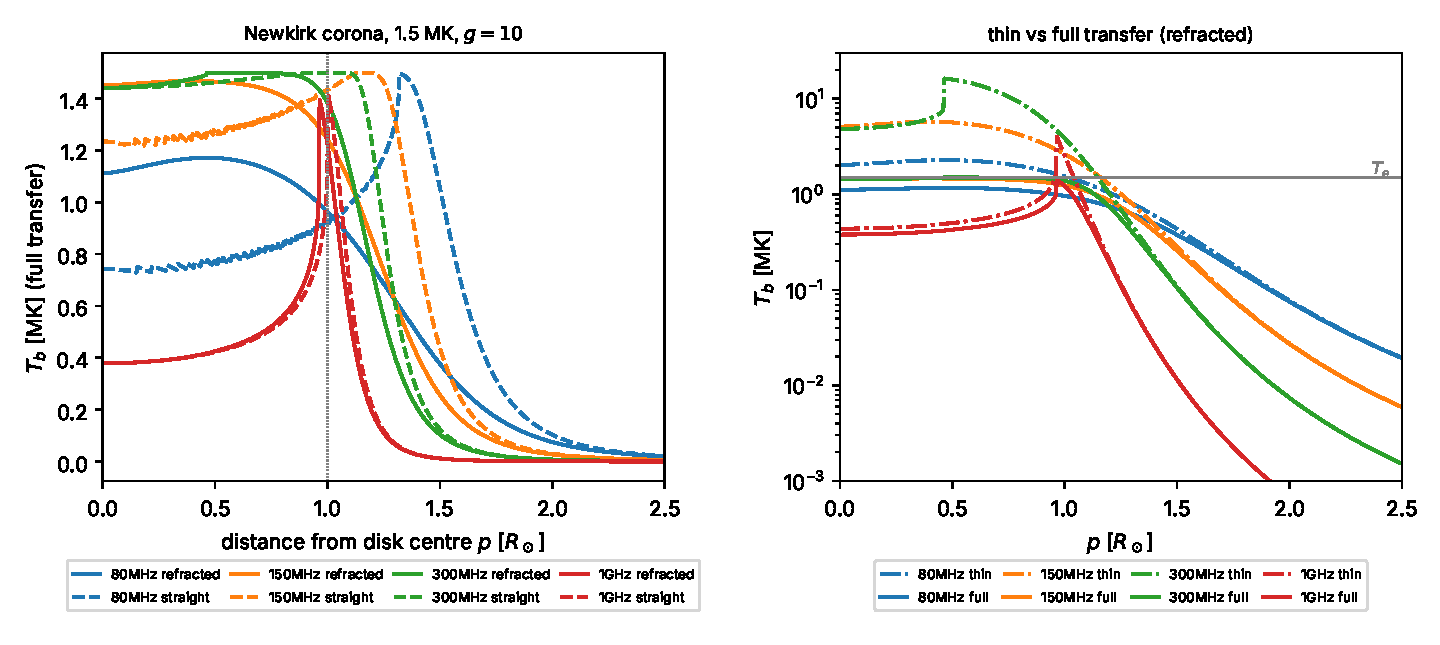
\includegraphics[width=\textwidth]{ff_profiles.pdf}
\caption{The result for a simple model corona at 1.5\,MK: brightness temperature from the centre
of the disk ($p=0$) outwards. Left: with refraction (solid) and with straight rays (dashed).
Right: full transfer (solid) and the thin sum (dash-dotted), which overshoots $T_e$.}
\label{fig:profiles}
\end{figure}

For the model corona of Fig.~\ref{fig:profiles}, the code finds at 80\,MHz a disk of about
1\,MK that extends beyond the visible Sun, and a total flux of about 3\,sfu --- close to what
radio telescopes see from the quiet Sun. At 1\,GHz the corona has become nearly transparent: the
disk is the size of the optical Sun, fainter in the centre and brighter at the limb, where the line
of sight through the corona is longest.

\keyidea{$T_b$ tells us the temperature of the layer we see; the sum over pixels gives the flux.}

%----------------------------------------------------------------------
\chapterhead{7.\quad What the lens changes}{Refraction on or off}

\textsf{radiosynth} can switch refraction off (\code{no\_refraction=True}) and compare the two
images (\code{rs.compare\_refraction}). Fig.~\ref{fig:profiles} (left) shows what happens at low
frequency. With refraction the radio Sun is \emph{smaller}, because rays that pass near the limb are
bent away and see less dense plasma (3.1 instead of 4.1\,sfu at 80\,MHz). Its centre, however, is
\emph{brighter}: a straight ray stops at the critical surface before the gas has become opaque,
while a bent ray turns above it and spends a long time in the dense plasma, so it collects more
light. At 1\,GHz the density is far below $\ncr$, the lens is gone, and both images agree.

\keyidea{refraction shrinks the low-frequency radio Sun and changes its brightness; at high
frequency it does not matter.}

%----------------------------------------------------------------------
\chapterhead{8.\quad The whole story in five lines}{}

\begin{enumerate}[label=\textbf{\arabic*.}]
\item For each pixel, start a ray at the telescope and send it into the model.
\item Bend it with the refractive index $\mu=\sqrt{1-n_e/\ncr}$, in small, controlled steps.
\item At each step, the gas glows at $B_\nu\propto T_e$ and absorbs at $\kappa_\nu\propto n_e^2\nu^{-2}T_e^{-3/2}$.
\item Add the glow of each step, dimmed by the gas in front: $I\leftarrow I+B(1-e^{-\Delta\tau})e^{-\tau}$.
\item Convert to $T_b$ and sum the pixels to get the flux.
\end{enumerate}

In \textsf{radiosynth} all of this is one line:
\begin{small}
\begin{verbatim}
img = rs.make_radio_image(grid, "80MHz, 150MHz, 1GHz", transfer="full")
\end{verbatim}
\end{small}
and the details, with every equation and the code that implements it, are in the companion note
\emph{Thermal free--free (bremsstrahlung) emission in radiosynth}.

\vspace{6pt}
{\small\textbf{Further reading.} Benkevitch et al.\ 2010, ApJ 725, 447 (the ray-tracing
algorithm); Moschou et al.\ 2018, ApJ 867, 51 (radio images from MHD models); Dulk 1985, ARA\&A 23,
169 (radio emission from the Sun and stars).}

\end{document}
